\documentclass[11pt, a4paper]{article}
\usepackage[spanish]{babel}
\usepackage[utf8]{inputenc}
\usepackage{mathpazo}
\usepackage{geometry}
\geometry{a4paper,
  left=1.2in,
  right=1.2in,
  top=1.2in,
  bottom=1.2in
}
\usepackage{titlesec}
\usepackage{fancyhdr}
\usepackage{setspace}
\usepackage{graphicx}
\usepackage{float}
\usepackage{microtype}

\pagestyle{fancy}
\fancyhf{}
\renewcommand{\headrulewidth}{0.8pt}
\fancyfoot[C]{\thepage}
\fancyhead[L]{\nouppercase{\rightmark}}
\fancyhead[R]{\nouppercase{Proyecto de LaTeX}}

\onehalfspacing

\setlength{\parskip}{1.8em}

\newcommand{\ensayoTitulo}[2]{%
  \begin{center}
    \vspace*{1cm}
    {\fontsize{36}{38}\selectfont\textbf{#1}} \\
    \vspace{0.4cm}
    {\fontsize{18}{20}\selectfont\textit{#2}}
    \vspace*{1.5cm}
    \hrule
    \vspace*{0.3cm}
  \end{center}
}

\begin{document}

\ensayoTitulo{La Cruz Griega de la Adición:}{Un Símbolo con Historia y Significado en el Lenguaje Matemático}

Adentrarse en el estudio de los símbolos matemáticos constituye una invitación a desentrañar cómo la humanidad ha logrado representar y comunicar nociones de índole eminentemente abstracta. Dentro de la vasta y rica simbología que configura el universo matemático, el signo de la adición, universalmente reconocido como la cruz de ``más'' (+), se erige como un pilar fundamental. Su génesis y evolución reflejan de manera elocuente la perenne búsqueda de concisión y universalidad inherente al intrincado lenguaje de las matemáticas. De hecho, la obra ``El lenguaje de las matemáticas: historias de sus símbolos'', del distinguido autor Raúl Rojas González, se presenta como una guía inestimable que nos permite explorar cómo cada notación atesora su propia historia y sus variaciones, enriqueciendo así su significado intrínseco.

Previamente a la consolidación de esta cruz como estándar, la operación de adición era expresada mediante una diversidad de métodos, a menudo caracterizados por su escasa practicidad. Uno puede conjeturar la ambigüedad inherente al empleo de locuciones completas como ``y'' o ``plus'', o a la proliferación de abreviaturas que divergían notablemente entre los copistas y las distintas regiones geográficas. Superar esta fragmentación y alcanzar una unicidad era imperativo para el progreso de los cálculos y la eficiente transmisión del conocimiento matemático. La imperiosa necesidad de una notación que trascendiera las barreras lingüísticas y agilizara las operaciones fue, sin duda, el catalizador de su evolución. Resulta particularmente fascinante observar cómo el símbolo ``+'' parece tener sus orígenes en el siglo XV, derivado de la abreviatura de la palabra latina ``et'', cuyo significado es, precisamente, ``y''. Es plausible imaginar cómo los escribas, imbuidos de un afán de eficiencia, fueron estilizando progresivamente esta ``t'' hasta conferirle la forma de cruz que hoy nos es tan familiar. Esta transformación pudo haberse visto influenciada por las diversas morfologías de cruces ya presentes en la simbología de la época, tal como se puede apreciar en la Figura 1.

\begin{figure}[H]
    \centering
    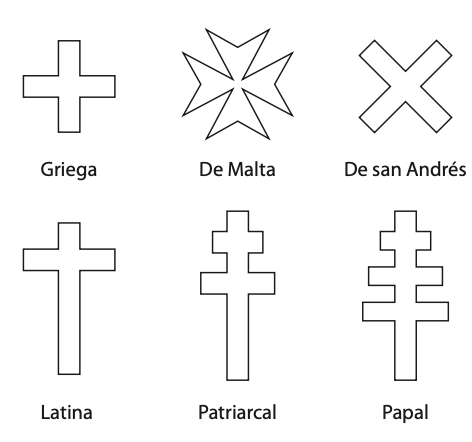
\includegraphics[width=0.7\textwidth]{Diversas cruces cristianas, inspiracion para simbolos matematicos..png}
    \caption{Diversas cruces cristianas, consideradas posibles influencias en la adopción de símbolos matemáticos (Rojas González, 2018, p. 83). Imagen recuperada del libro.}
    \label{fig:cruces}
\end{figure}

En este contexto histórico, Johannes Widmann, en su relevante tratado de aritmética comercial \textit{Mercantile Arithmetic} publicado en 1489, es frecuentemente reconocido como uno de los pioneros en emplear estos signos de adición y sustracción en un contexto impreso, si bien su adopción generalizada se efectuaría de manera gradual.

La asimilación de este símbolo, cabe señalar, no se consumó como un proceso inmediato ni homogéneo; durante un periodo considerable, coexistió con otras notaciones en diversas latitudes. No obstante, la inherente claridad visual que la cruz ofrecía, junto con su notoria economía de espacio, la tornaron, de modo ineludible, imprescindible. Su facilidad de reproducción, tanto en los manuscritos de la época como, crucialmente, en los incipientes sistemas de imprenta, desempeñó un papel determinante en su rauda difusión y subsiguiente hegemonía. Este proceso de estandarización es un vívido ejemplo de la progresiva abstracción que tan distintivamente caracteriza a las matemáticas. Al encapsular una operación conceptualmente compleja en un símbolo de simplicidad elemental, la cognición humana se libera, permitiendo una concentración más profunda en la estructura subyacente de los problemas y en las intrincadas relaciones entre las cantidades, más allá de la mera operatoria.

\vspace*{1 cm}
\begin{center}
    {\fontsize{24}{26}\selectfont\textbf{Conclusión Personal}}
\end{center}
\vspace*{0.8em}

Desde mi posición como estudiante que ha profundizado en este tema, con el apoyo del texto de Rojas González, el desarrollo del signo de adición es, sin duda, un hito significativo. Constituye un testimonio elocuente de la incesante búsqueda de eficiencia y universalidad que ha modelado el lenguaje matemático. La transición de expresiones verbales o abreviaturas ambivalentes a un símbolo tan conciso y diáfano como el ``+'' representa, a mi juicio, un avance verdaderamente paradigmático. Lo que más aprecio de esta notación es su simplicidad intrínseca y su reconocimiento global, factores que facilitan la comprensión del concepto de adición sin imponer barreras lingüísticas. Sinceramente, si se me pidiera sugerir alguna modificación, me resultaría arduo proponerla, pues su eficacia reside precisamente en esa pureza y sencillez. Este símbolo encarna, en su esencia, una solución elegante y perdurable a la necesidad fundamental de comunicar una operación básica. Reafirma cómo la innovación en la notación es inseparable del progreso del pensamiento matemático y de su asombrosa capacidad para trascender el tiempo y las diversas culturas. La obra de Rojas González nos invita, en cada página, a valorar que incluso los elementos más fundamentales del lenguaje matemático poseen profundas raíces históricas y culturales, conectándonos con siglos de ingenio en cada aplicación que les conferimos.

\newpage

\begin{thebibliography}{99}
    \bibitem{Rojas2018} Raúl Rojas González. (2018). \textit{El lenguaje de las matemáticas. Historias de sus símbolos}. Fondo de Cultura Económica. Capítulo consultado: “Operadores aritméticos”, pp. 82–86. Imagen de la Figura 1 (p. 83) recuperada del libro.
\end{thebibliography}

\end{document}